\subsection{Data Retrieval mit Apache Zeppelin}
Apache Zeppelin bringt standardmäßig einige nützliche Funktionen mit, die es für die Datenauswertung interessant machen. Dazu zählen u.A.:
\begin{itemize}
	\item SQL via JDBC inkl. PostgreSQL Support
	\item Interaktive Diagramme über Formulargeneriung und Pivot-Charts
	\item Frei konfigurierbare Anordnung der Diagramme im Notebook
	\item Versionsverwaltung für Notebooks um verschiedene Stände abzuspeichern und schnell zwischen Versionen zu wechseln
\end{itemize}

Über den Befehl \shellcmd{/bin/zeppelin.sh} startet Zeppelin und ist standardmäßig im Browser über den Port 8080 erreichbar. Die gesamte Konfiguration, Entwicklung und Ausführung des Notebooks erfolgt im Web. Letztlich ist ein Notebook ein Kanvas in den man Kacheln erstellen und verwalten kann. Jede Kachel besteht aus 3 integralen Bestandteilen:
\begin{itemize}
	\item \textbf{Code} der mittels der vielen Interpreter die Daten läd, die angezeigt werden sollen, z.B. SQL.
	\item \textbf{Konfiguration} der Visualisierung. Dazu zählen verschiedene Diagrammtypen und -konfigurationen sowie generierte Formularfelder. 
	\item \textbf{Diagramm} welches die Daten responsiv visualisiert oder eine schlichte Tabelle um die Daten darzustellen.
\end{itemize}

Sobald der Code ausgeführt wird, egal ob manuell oder per automatischen Zyklus, wird das Diagramm in der Kachel aktualisiert.


Leider ist die Auswahl an Diagrammtypen und deren Flexibilität und Erfassbarkeit abhängig von den Daten sehr begrenzt. Standardmäßig gibt es nur eine schlichte Tabelle, Balken-, Flächen-, Linien- und Punktdiagramm die relativ starr sind. Da erweiterte Visualisierungen wie Heatmaps und Karten noch in der Entwicklung sind ist die Auswertung auf die oben genannten Typen begrenzt. Zudem ist die maximale Anzahl an Datensätzen die dargestellt bzw. visualisiert werden könne auf 102400 begrenzt. Nichts desto trotz wurde ein beispielhaftes Notebook erstellt:

\begin{figure}[h] 
	\centering
	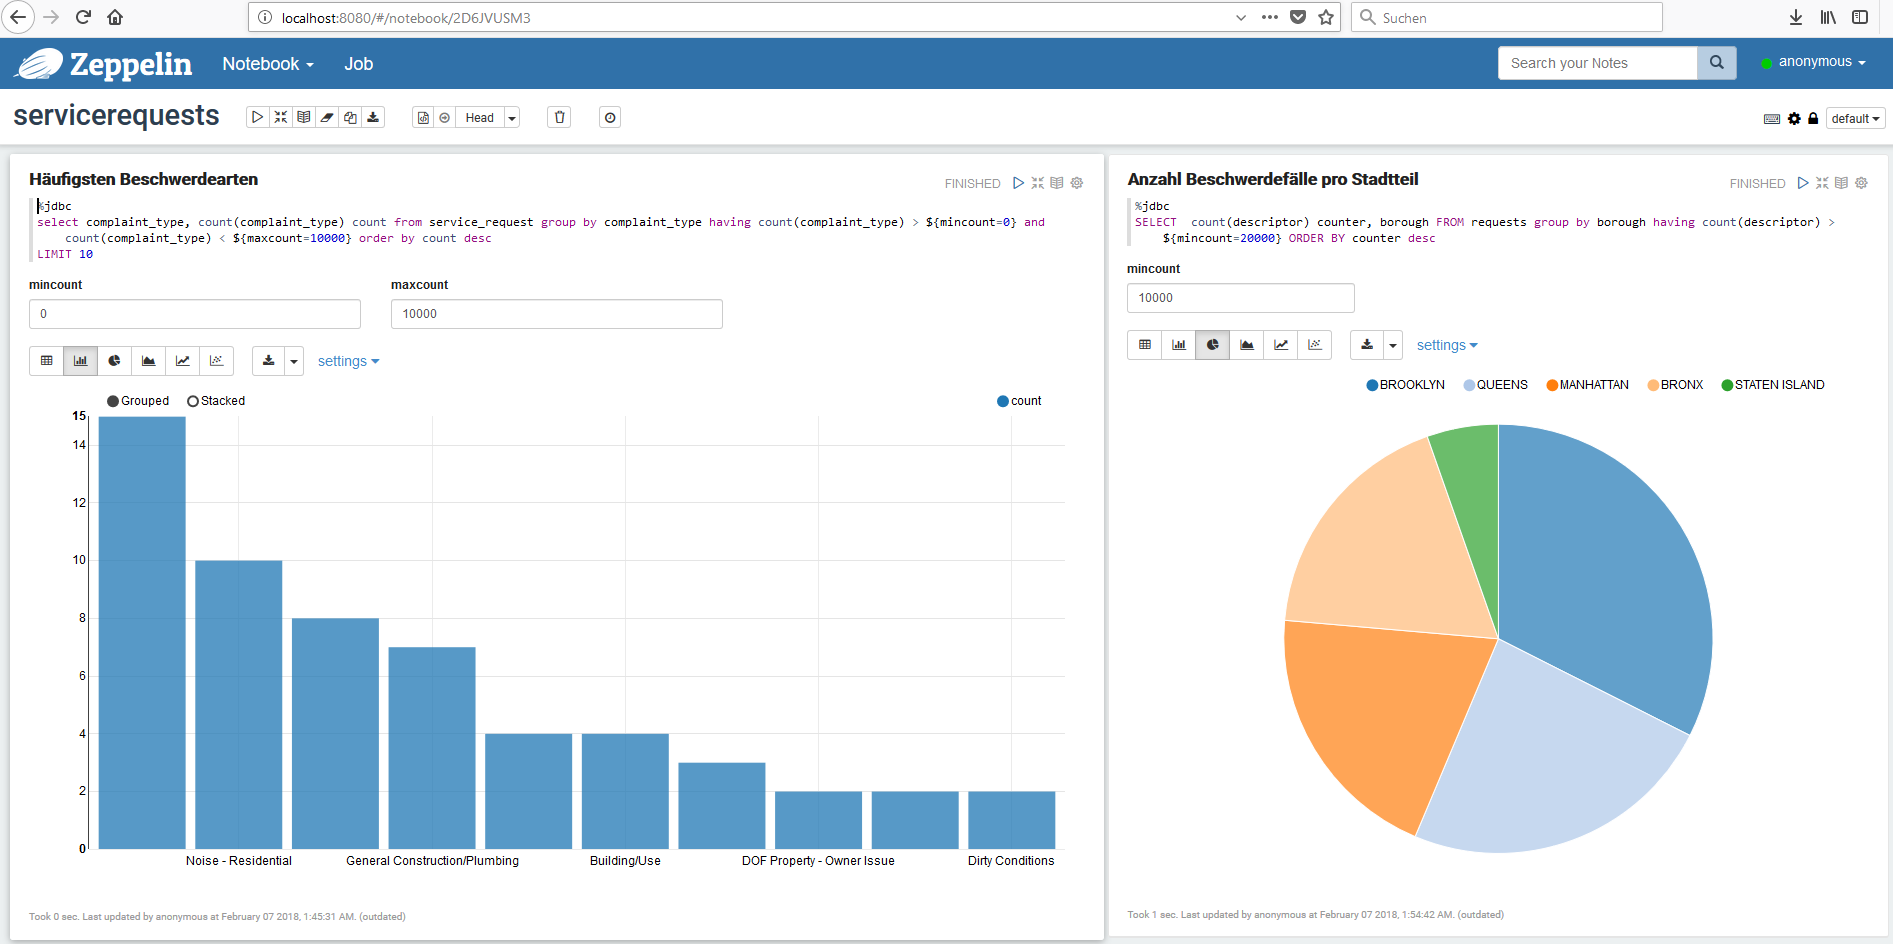
\includegraphics[width=\linewidth]{dualComplainChart.png}
	\caption[Ausschnitt des Notebooks]{Ausschnitt des Zeppelin Notebooks}
	\label{fig:zeppelin1}
\end{figure}
%\begin{figure}[h] 
%	\centering
%	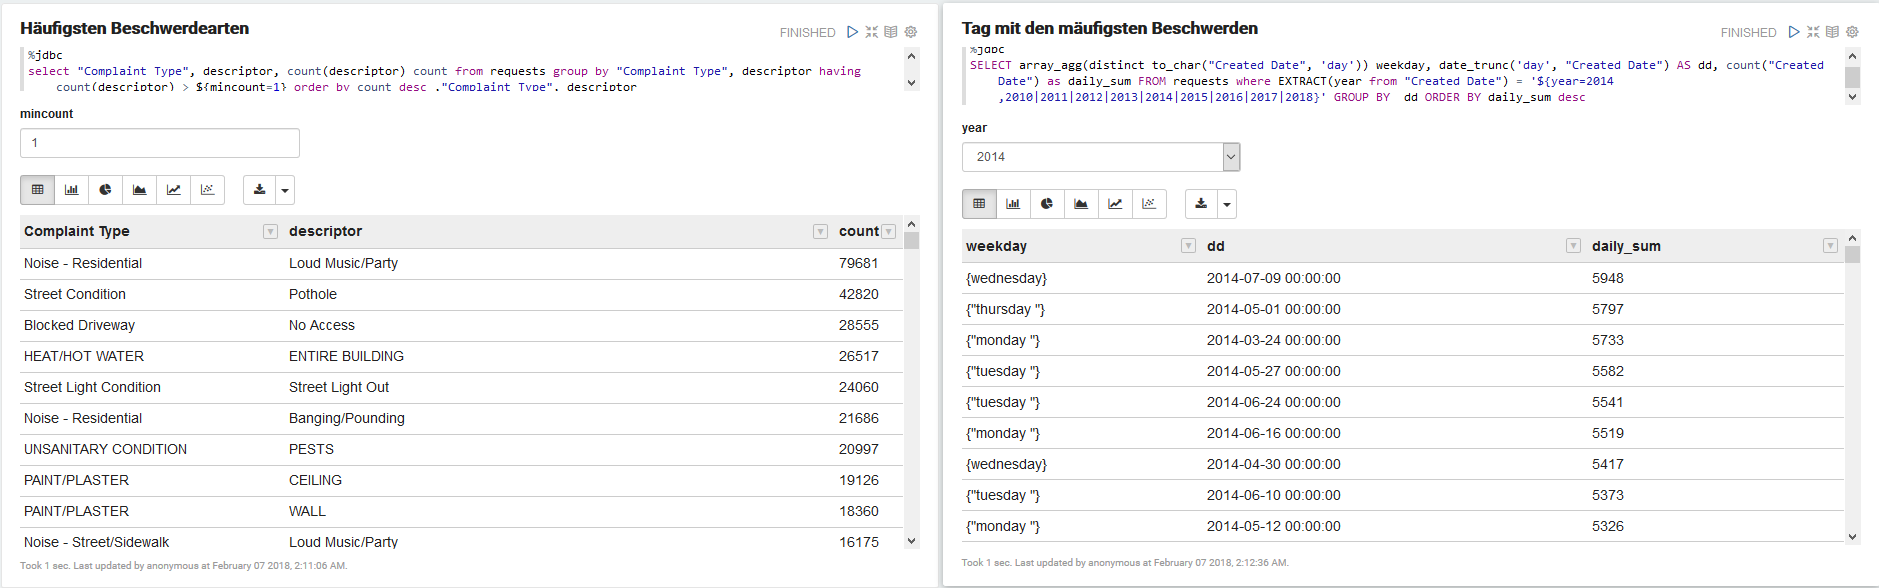
\includegraphics[width=\linewidth]{dualComplainDaychart.png}
%	\caption[Ausschnitt des Notebooks]{Ausschnitt des Notebooks}
%	\label{fig:zeppelin2}
%\end{figure}
\begin{figure}[h] 
	\centering
	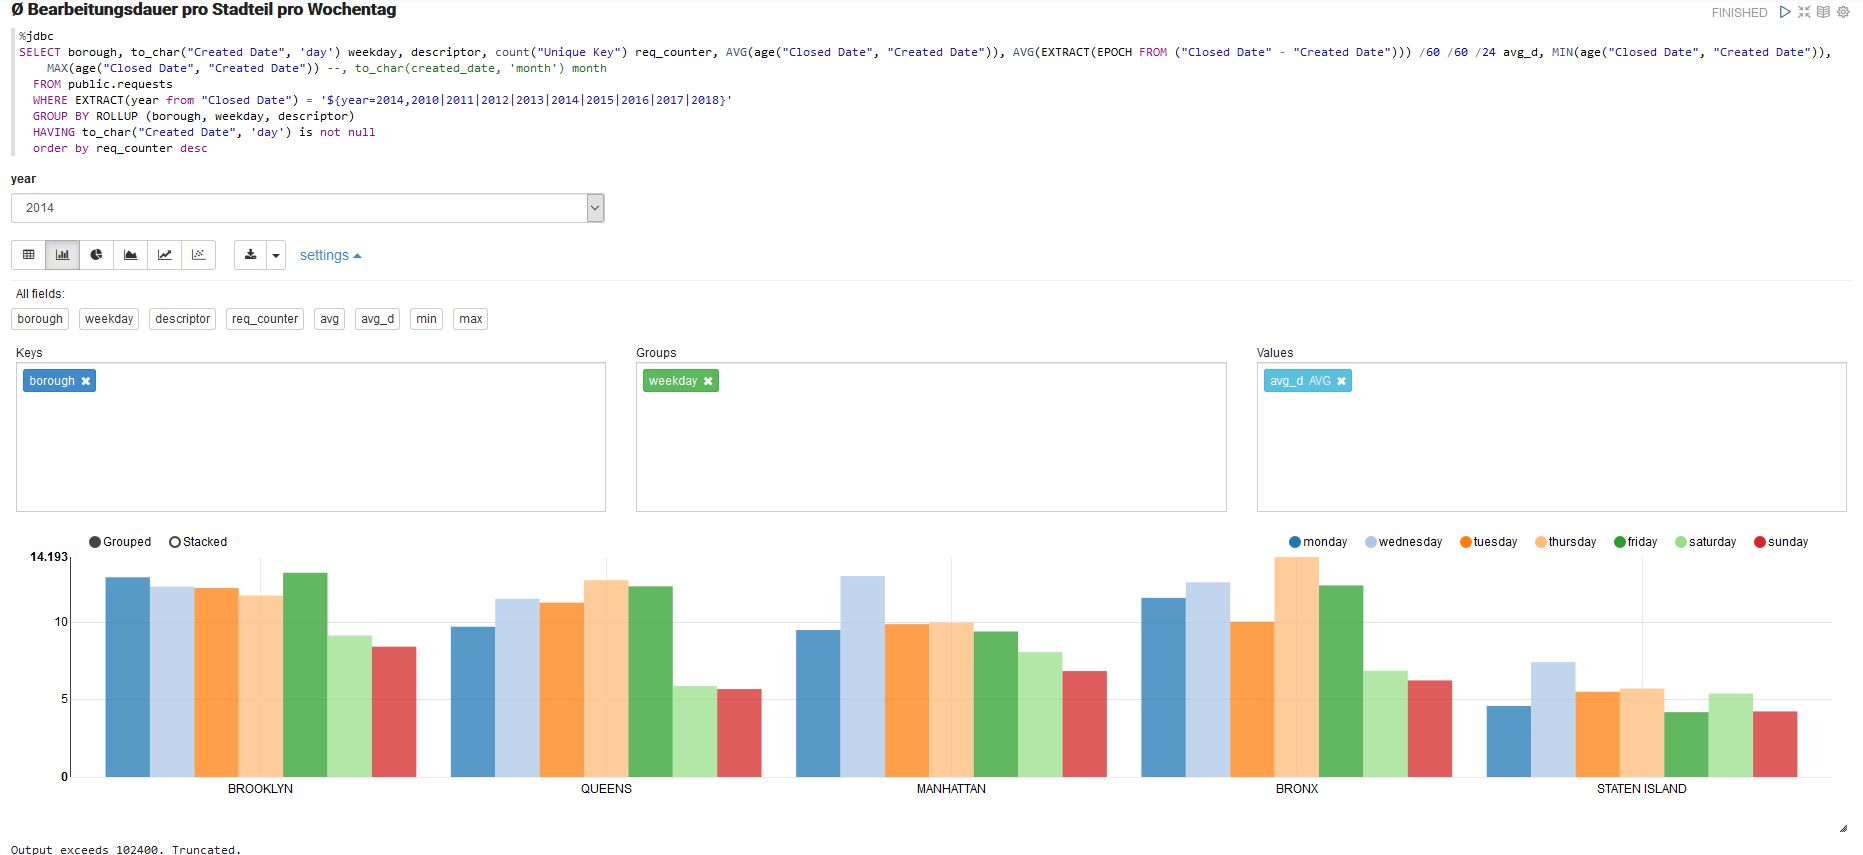
\includegraphics[width=\linewidth]{comByRegion.png}
	\caption[Pivot Chart im Zeppelin Notebook]{Pivot Chart im Zeppelin Notebook}
	\label{fig:zeppelin3}
\end{figure}


